\documentclass[ignorenonframetext,xcolor=x11names]{beamer}

\input{../common.preamble.beamer.tex}
 
\title{Business 4720 - Class 2}

\subtitle{Data Types and Data Sources}

\begin{document}

\begin{frame}{}
  \titlepage
  \footnotesize
  \input{../license.tex}
\end{frame}

\section{Introduction}

\begin{frame}{This Class}

\begin{block}{What You Will Learn:}
\begin{itemize}
  \item Different data types
  \item Data quality and provenance
  \item Internal and external data sources
\end{itemize}
\end{block}
\end{frame}

\section{Data Types}

\begin{frame}{Primitive Data Types}
\small
\renewcommand{\arraystretch}{1.25}

\begin{tabularx}{\textwidth}{l|X} \hline
char 			& Individual Characters\\
string			& A string of characters\\
byte			& 1 byte, $-128 \ldots 127$ or one Ascii characters \\
int (16 bit)	& ''Short'', Integer numbers, $-32,768 \ldots 32,767$ \\ 
int (32 bit)	& ''Long'', Integer numbers, $-2,147,483,648 \ldots 2,147,483,647$ \\
int (64 bit)	& Integer numbers, $-9,223,372,036,854,775,808 \ldots$ $9,223,372,036,854,775$ \\
float			& Decimal numbers, 6 to 7 significant digits \\
double			& Decimal numbers, 15 to 16 significant digits \\
boolean			& Logical, true/false, 1 or 0 \\ \hline
\end{tabularx} \\
\vspace{5mm} \\
Not all tools use the same names, and not all tools make the same distinctions. For example, the R system uses \texttt{numeric} (which is actually a double type) and \texttt{integer} (which is a 32 bit integer).
\end{frame}

\begin{frame}{Missing Values}
\begin{itemize}
	\item Depends on software tool
	\item Different meanings (such as not applicable, not available)
\end{itemize}

\centering
\vspace{5mm}
\renewcommand{\arraystretch}{1.25}

\begin{tabular}{l|l} \hline
R &	NA \\
Python & None \\
SQL & Null \\ \hline
\end{tabular}
\end{frame}

\begin{frame}{Floating Point Numbers (IEEE 754 Standard)}
\includegraphics[width=\textwidth]{IEEE754.png}
\tiny
\url{https://commons.wikimedia.org/wiki/File:IEEE_754_Double_Floating_Point_Format.svg}
\normalsize

\begin{align*}
& (-1)^{\text{sign}} ( 1.b_{51}b_{50} \ldots b_0)_2 \times 2^{\text{exp}-1023} \\
& (-1)^{\text{sign}} \left( 1 + \sum_{i=1}^{52} b_{52-i}2^{-i} \right) \times 2^{\text{exp}-1023}
\end{align*}

\footnotesize
\renewcommand{\arraystretch}{1.25}

\begin{tabularx}{\textwidth}{l|X} \hline
float			& 4 bytes, 1 bit for sign, 8 bits for exponent, 23 bits for significand, $\pm 3.40282347e+38$ \\
double			& 8 bytes, 1 bit for sign, 11 bits for exponent, 52 bits for significand, $\pm 1.79769313486231570e+308$ \\ \hline
\end{tabularx}
\end{frame}

\begin{frame}{Floating Point Serialization to Text}
\begin{block}{Idiosyncrasies}
\begin{itemize}
	\item Thousands separator, grouping
	\item Negatives in brackets
	\item ''Scientific notation''
\end{itemize}
\end{block}

\footnotesize
\centering
\vspace{5mm}
\renewcommand{\arraystretch}{1.25}

\begin{tabular}{r|l} \hline
-1023476.56 & \\
-1023476,56 & some locales use comma as decimal sep \\
-1,023,476.56 & some locales use comma for grouping \\
-1.023.475,56 & some locales use comma as sep and points to group \\
(1,023,476.56) & some applications use brackets for neg \\
-1 023 476.56 & some locales use space for grouping \\
-1.02347656e+06 & ''scientific notation'' \\
-1023.47656e+03 & also ''scientific notation'' \\
$\ldots$ & \\ \hline
\end{tabular}
\end{frame}

\begin{frame}[fragile]{Characters (Unicode ISO/IEC 8859)}
\begin{itemize}
	\item Covers all major alphabets and writing systems
	\item 149,813 symbols (V15.1), incl 3782 emojis, for 161 scripts
\end{itemize}
\begin{block}{UTF-8}
\small
\begin{itemize}
	\item Most widely used Unicode encoding standard
	\item Standardized 1998 as RFC 2277
	\item 1 to 4 byte variable length encoding for each character
	\item Initial 127 bytes backwards compatible with ASCII character set
\end{itemize}
\end{block}

\footnotesize
\begin{minted}[bgcolor=code,frame=single,framesep=5pt,escapeinside=||]{text}
Roman alphabet: Inuktitut
Written Inuktitut: |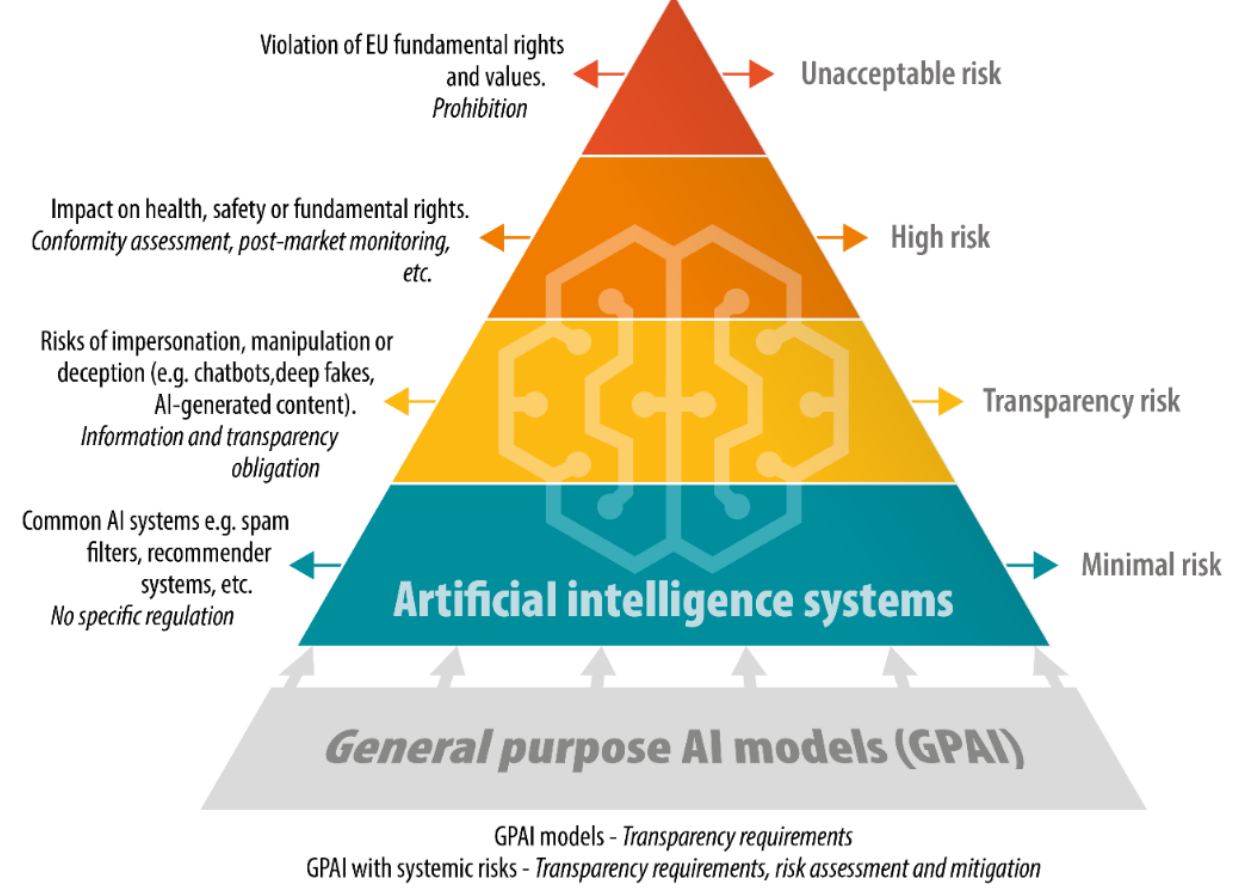
\includegraphics[height=14pt]{screen2.png}|
Unicode characters: \u1403 \u14c4 \u1483 
                    \u144e \u1450 \u1466
UTF-8 Encoding: 0xE1 0x90 0x83 0xE1 0x93 0x84 
                0xE1 0x92 0x83 0xE1 0x91 0x8E 
                0xE1 0x91 0x90 0xE1 0x91 0xA6
\end{minted}

\end{frame}

\begin{frame}{Unicode}
\centering

\includegraphics[height=3.25in]{weird_unicode_math_symbols.png} \scriptsize Source: \url{https://xkcd.com} (CC license)

\end{frame}

\begin{frame}{Hands-On Exercise}
\begin{itemize}
	\item Choose your favourite emoji
	\item Determine its Unicode number (''codepage'')
	\item Determine its UTF-8 encoding
\end{itemize}
\end{frame}

\begin{frame}{Dates and Times}
\begin{block}{Complexities}
\begin{itemize}
   \item Calendar formats (written)
   \begin{itemize}
		\item DMY, YMD, MDY, YDM with different separators (''.'', ''-'', ''/'')
		\item Not all software or data sets comply with standards
		\item Difficult to parse and validate
	\end{itemize}
   \item 12 hour (AM/PM) and 24 hour time formats
   \item Time zones
   \item Leap seconds, leap years
   \item Week numbering
   \item Precision (milliseconds, nanoseconds)
   \item Different written formats
   \item Arithmetic involving years, months, days
\end{itemize}
\end{block}
\end{frame}

\begin{frame}{Dates and Times}
\centering
\includegraphics[width=\textwidth]{datetime.png} 

\scriptsize Source: \url{https://xkcd.com} (CC license)
\end{frame}

\begin{frame}{ISO 8601 and RFC 3339 Date Format} 
\footnotesize
\renewcommand{\arraystretch}{1.25}

\begin{tabular}{l|l} \hline
	Calendar dates & YYYY-MM-DD  \\ \hline
	\textit{Ordinal dates} & \textit{YYYY-DDD} (not in RFC 3339) \\ \hline
	\textit{Week dates} & \textit{YYYY-Www-d} (not in RFC 3339) \\ \hline
	\multirow{5}{*}{Times} & Thh:mm:ss.sss \textit{(or Thhmmss.ss)} \\
	& Thh:mm:ss \textit{(or Thhmmss)} \\
	& \textit{Thh:mm.mmm or Thhmm.mmm} \\
	& \textit{Thh:mm or Thhmm} \\
	& \textit{Thh.hhh} \\ \hline
	\multirow{2}{*}{Time Zones} & <time>Z or <time>$\pm$hh:mm or \\
	& \textit{(<time>$\pm$hhmm or <time>$\pm$hh)} \\ \hline
	Combined & <date>T<time> \\
	Periods & PnYnMnDTnHnMnS or P<date>T<time>
\end{tabular}
\begin{block}{Leap Year Rule}
(year \% 4 == 0) and (year \% 100 != 0 or year \% 400 == 0)
\end{block}
\end{frame}

\begin{frame}{Hands-On-Exercises}

\begin{tcolorbox}[colback=code]
The territory of Nunavut was created on April 1st, 1999.
\end{tcolorbox}

\begin{itemize}
	\item Express the date in RFC 3339
	\item Calculate the number of days since the creation of Nunavut
	\item Assume that a ceremony took place at 3PM that day in Iqaluit and express this date-time in RFC 3339
	\item Assume the ceremony lasted for 125 minutes and express this duration in RFC 3339
\end{itemize}
\end{frame}

\begin{frame}{Complex/Structured Data Types}
\small
\begin{block}{Python}
	\begin{itemize}
		\item list, \texttt{[1, 2, "a", "b", 2]}, mutable, ordered
		\item tuple, \texttt{(1, 2, "a", "b", 2)}, immutable
		\item set, \texttt{\{1, 2, "a", "b"\}},  mutable, unordered
		\item dict, \texttt{\{"make": "Ford", "year": 2023\}}, mutable
	\end{itemize}
\end{block}
\begin{block}{R}
	\begin{itemize}
		\item list, \texttt{list(1, 2, "a", "b", 2)}, mutable, ordered
		\item vector, \texttt{c(1, 2, 3)}, mutable, same primitive type
		\item factor, \texttt{as.factor(c("Hot", "Med", "Cold"))}
		\item matrix, \texttt{matrix(c(1, 2, 3, 4), nrow=2)}
		\item array, \texttt{array(c(1, 2, 3), c(4, 5, 6))}
	\end{itemize}
\end{block}
\end{frame}

\section{Structured Data Types}

\begin{frame}{Data Types in Analytics}
\begin{block}{Structured Data}
\begin{itemize}
	\item Tables
	\item Key-Value pairs
	\item Documents (JSON, XML)
	\item Graphs
\end{itemize}
\end{block}
\begin{block}{Unstructured Data}
\begin{itemize}
	\item Text
	\item Image
	\item Video
\end{itemize}
\end{block}
\end{frame}

\begin{frame}{Tables}
\begin{itemize}
	\item Columns, represent different variables
		\begin{itemize}
			\item Each column is a vector, typically named
		\end{itemize}
	\item Rows, represents values for different observations
	\item Cells, may be primitive or complex, e.g. sets or lists or tables
\end{itemize}
\centering
\vspace{5mm}
\renewcommand{\arraystretch}{1.25}

\begin{tabular}{l|r|r} \hline
\textbf{Name} & \textbf{Area} & \textbf{Population} \\ \hline
Canada & 9,984,670 & 38,781,292  \\
Nigeria & 923,768 & 223,804,632 \\
Germany & 357,600 & 83,294,633 \\ \hline
\end{tabular}
\end{frame}

\begin{frame}[fragile]{Table Interchange/Serialization}
\begin{block}{CSV format (RFC 4180)}
\begin{itemize}
	\item Plain text, Ascii or UTF-8 Unicode
	\item One record per line
	\item Fields separated by delimiter (typically: '','')
	\item Fields must be primitive
	\item Optional header with column/field names
	\item Fields \emph{may} be enclosed by double quotes ('' " '')
\end{itemize}
\end{block}

\begin{minted}[bgcolor=code,frame=single,framesep=10pt]{text}
"Name", "Area", "Population" <LF>
"Canada", "9984670", "38781292" <LF>
"Nigeria", "923768", "223804632" <LF>
"Germany", "357600", "83294633" <LF>
\end{minted}
\end{frame}

\begin{frame}{Table Interchange/Serialization \small [cont'd]}
\begin{block}{Potential Problems with CSV Files}
\begin{itemize}
	\item Different delimiters ('','', ''tab'', '';'', ''{ }\^{} '', etc.)
	\item Different line endings/terminators (CR/LF for Windows, LF for Mac \& Unix)
	\item Different or inconsistent quoting
	\item Different decimal and thousand delimiters for numerics (depending on locale)
	\item Different date formats (depending on locale)
\end{itemize}
\end{block}
\end{frame}

\begin{frame}{Hands-On Exercise}
\begin{itemize}
	\item Search the internet for a CSV file of the population and areas of all countries of the world
	\item Examine the CSV file and answer the following questions:
	\begin{itemize}
		\item What is the delimiter?
		\item Which fields are quoted, and how?
		\item What is the line ending character(s)?
		\item What is the number format?
		\item What is the date format (if there are dates)?
	\end{itemize}
	\item Import the CSV file into your favourite spreadsheet tool
	\begin{itemize}
		\item Does it recognize all information correctly? If not, what is not imported well?
	\end{itemize}
	\item Export the CSV file from your tool under a different name.
	\begin{itemize}
		\item Do you get an identical file to the one you imported? If not, what has changed?
	\end{itemize}
\end{itemize}
\end{frame}

\begin{frame}{Relational Databases}
\begin{block}{Characteristics}
\begin{itemize}
	\item Records (''rows'') in tables (''relations'')
	\item Columns/fields are typed
	\item Records are identified by ''primary keys''
	\item Records can refer to other records, in the same or different relation/table
\end{itemize}
\end{block}
\centering
\includegraphics[height=1.5in]{Relational_key.png}
\tiny{\url{https://commons.wikimedia.org/wiki/File:Relational_key_SVG.svg}}
\end{frame}

\begin{frame}{Relational Databases \small [cont'd]}
\begin{block}{Advantages}
\begin{itemize}
	\item Normalization reduces redundancy, increases data integrity
	\item Enforcement of contraints such as types, referential integrity, non-nulls, etc. increases data integrity
	\item Intuitive schemas and queries
\end{itemize}
\end{block}

\begin{block}{Prominent Examples}
\begin{itemize}
	\item \emph{On-premises}: Oracle DBMS
	\item \emph{Open source}: PostgreSQL
	\item \emph{Cloud}: Amazon RDS, Google Cloud Database, Azure SQL
\end{itemize}
\end{block}
\end{frame}

\begin{frame}{Key-Value Data Stores}
\begin{block}{Characteristics}
\begin{itemize}
	\item Records are sets of key-value pairs
	\item Key has multiple components (ordered list, ''minor keys'')
	\item Value is uninterpreted
\end{itemize}
\end{block}
\centering
\includegraphics[height=1.5in]{KeyValue.png}
\tiny{\url{https://commons.wikimedia.org/wiki/File:KeyValue.PNG}}
\end{frame}

\begin{frame}{Key-Value Data Stores \small [cont'd]}
\begin{block}{Advantages}
\begin{itemize}
	\item Fast retrieval/insertion/updating
	\item No relationships between entities/records
	\item Less memory use (does not store empty table cells)
	\item Untyped and no fixed schema increases flexibility
	\item Easy scalability and distribution
\end{itemize}
\end{block}
\begin{block}{Prominent Examples}
\begin{itemize}
	\item \emph{On-premises, open-source}: Apache Cassandra, Facebook RocksDB, Redis
	\item \emph{Cloud}: AWS DynamoDB, Google LevelDB, Azure CosmosDB
\end{itemize}
\end{block}
\end{frame}

\begin{frame}{Documents (JSON)}
\begin{block}{JavaScript Object Notation (RFC 8259)}
\begin{itemize}
	\item Plain text, UTF-8 
	\item Primitive Types:
	\begin{itemize}
		\item Strings (in single or double quotations)
		\item Number
		\item Boolean
		\item Null
	\end{itemize}
	\item Structured Types:
	\begin{itemize}
		\item Objects
		\begin{itemize}
			\item unordered collection of zero or more name/value pairs)
			\item Delimited by ''\{'' and ''\}''
		\end{itemize}
		\item Arrays
		\begin{itemize}
			\item Ordered sequence of zero or more values
			\item Delimited by ''['' and '']''
		\end{itemize}
	\end{itemize}
\end{itemize}
\end{block}
\end{frame}

\begin{frame}[fragile]{JSON Example -- Complex Object}
\footnotesize
\begin{minted}[bgcolor=code,frame=single,framesep=10pt]{json}
{
  "Image": {
    "Width": 1060,
    "Height": 400,
    "Title": "Skyline of Iqualuit, Nunavut",
    "Url": 
"https://upload.wikimedia.org/wikipedia/commons/b/b4/Iqaluit_skyline.jpg",
    "Legal": {
      "Copyrighted": true,
      "License": "GNU Free Documentation License",
      "Inception": "2010-03-24",
      "Author": "Aaron Lloyd"
     },
  }
}
\end{minted}
\end{frame}

\begin{frame}[fragile]{JSON Example -- List of Objects}
\footnotesize
\begin{minted}[bgcolor=code,frame=single,framesep=10pt]{json}
[
  {
    "Latitude":  56.536389,
    "Longitude": -61.718889,
    "City":      "Nain",
    "Province":  "NL",
    "Postal":    "A0P",
    "Country":   "Canada"
  },
  {
    "Latitude":  53.512778,
    "Longitude": -60.135556,
    "City":      "Sheshatshiu",
    "Province":  "NL",
    "Postal":    "A0P",
    "Country":   "Canada"
  }
]
\end{minted}
\end{frame}

\begin{frame}{Hands-On Exercise}
\begin{block}{Document yourself in a JSON object}
\begin{itemize}
	\item Identify information about yourself, such as names, addresses, dates, relationships (work, school, uni), etc.
	\item Structure the information in JSON Objects and Arrays 
	\item Use nested structures, e.g. objects in arrays, or arrays in objects, or objects in objects, etc.
\end{itemize}
\end{block}
\end{frame}

\begin{frame}[allowframebreaks]{Document Databases}
\begin{block}{What makes them special}
\begin{itemize}
	\item \emph{Nested} key-value data store
	\item All keys are \emph{strings}
	\item No fixed schema, increases flexibility
\end{itemize}
\end{block}

\begin{block}{Applications}
\begin{itemize}
	\item Content management
	\item Catalogs and product data
	\item Log and event data (IoT, sensors)
\end{itemize}
\end{block}

\begin{block}{Prominent Examples}
\begin{itemize}
	\item \emph{On-premises}: MongoDB, ArangoDB
	\item \emph{Open source}: Apache CouchDB
	\item \emph{Cloud}: AWS DocumentDB, Azure CosmosDB
\end{itemize}
\end{block}
\end{frame}

\begin{frame}{Extensible Markup Language -- XML}
\begin{itemize}
   \item Document serialization format for structured data
   \item Nested \textbf{elements}
   \item Elements described by opening and closing \textbf{tag}
   \item Elements may have \textbf{attributes}, defined in opening tag
   \item Attributes can only hold simple data, elements can contain structured data.
   \item Arbitrary element and attribute names unqiuely defined within \textbf{namespaces} (typically URI, Uniform Resource Identifier)
   \item Element and attribute are defined using \textbf{XML Schema}
\end{itemize}
\end{frame}

\begin{frame}[fragile]{XML Example}
\begin{xmlcode}
<People
      xmlns="https://www.example.com/peoples"
      xmlns:geo="http://www.example.com/geo" 
      xmlns:hist="http://www.example.com/history">
    <GeneralInformation 
            Name="Innu" Language="Innu-aimun">
        <geo:Location geo:Country="Canada" 
                  geo:Regions="Labrador, Quebec" />
    </GeneralInformation>
    <hist:History>
        <hist:Period hist:era="Pre-Colonial">
            <Description>
                Nomadic lifestyle, primarily 
                hunting and fishing.
            </Description>
        </hist:Period>
\end{xmlcode}
\end{frame}

\begin{frame}[fragile]{XML Example \small [cont'd]}
\begin{xmlcode}
        <hist:Period hist:era="Post-Colonial">
            <Description>
                Impact of colonization, 
                including displacement and 
                cultural changes.
            </Description>
        </hist:Period>
    </hist:History>
    <Culture>
        <Traditions>
            <Tradition>
                Hunting and fishing as cultural 
                and subsistence activities.
            </Tradition>
            <Tradition>
                Use of the tepee for temporary 
                shelter.
            </Tradition>
        </Traditions>
\end{xmlcode}
\end{frame}

\begin{frame}[fragile]{XML Example \small [cont'd]}
\begin{xmlcode}
        <Art>
            <Form>Drum making</Form>
            <Form>Clothing with intricate beadwork
            </Form>
        </Art>
    </Culture>
    <Challenges>
        Issues like land rights, cultural preservation
    </Challenges>
</People>
\end{xmlcode}
\end{frame}

\begin{frame}{XML Example -- Key Points}
\small
\begin{itemize}
\item The \texttt{xmlns:geo} and \texttt{xmlns:hist} are namespace declarations. They are used to distinguish between geographical (geo) and historical (hist) data. Notice how element and attribute names may be prefixed by a namespace. 
\item The \texttt{xmlns} is the default namespace and applies to all elements and attributes without an explicit namespace.
\item The \texttt{GeneralInformation} element has attributes for Name and Language. Attributes must be character strings
\item The \texttt{Location} element includes attributes for Country and Regions, using the \texttt{geo} namespace.
\item The \texttt{Location} does not include other elements and is defined with just one tag.
\item Each \texttt{Period} element in the \texttt{History} element has an attribute \texttt{hist:era} to specify the era.
\item Multiple elements with the same name can follow each other.
\end{itemize}
\end{frame}

\begin{frame}[fragile]{Equivalent JSON Example}
\footnotesize
\begin{minted}[bgcolor=code,frame=single,framesep=10pt]{json}
{ "Innu": {
    "GeneralInformation": {
       "Location": {
         "Country": "Canada",
         "Regions": "Labrador, Quebec"
       }
    },
    "History": {
      "Period": [
        {
          "era": "Pre-Colonial",
          "Description": "Nomadic lifestyle, 
              primarily hunting and fishing."
        },
        {
          "era": "Post-Colonial",
          "Description": "Impact of colonization, ..."
        }
      ]
    },
\end{minted}
\end{frame}

\begin{frame}[fragile]{XML --- JSON}
\begin{itemize}
   \item Both are human and machine readable
   \item Both are system/language independent
   \item XML is more verbose/lengthy and very self-descriptive
   \item JSON is more compact/lightweight but not as descriptive
   \item XML supports more complex structures than JSON through
   \begin{itemize} 
      \item Attributes
      \item Namspaces
      \item More datatypes
   \end{itemize}
   \item XML can be strictly defined using XML Schema, JSON always remains flexible
\end{itemize}
\end{frame}

\begin{frame}{Hands-On Exercise}
\begin{block}{Document yourself in an XML document}
\begin{itemize}
	\item Identify information about yourself, such as names, addresses, dates, relationships (work, school, uni), etc.
	\item Structure the information in Elements and Attributes 
	\item Use nested elements where appropriate
\end{itemize}
\end{block}
\end{frame}

\begin{frame}{Graphs}
\begin{block}{Characteristics}
\begin{itemize}
	\item Nodes (also called ''vertices'')
	\item Edges (also called ''arcs'', ''relationships'') that connect vertices
	\begin{itemize}
		\item Directed or undirected
	\end{itemize}
	\item Vertices and Edges may be typed
\end{itemize}
\end{block}
\begin{block}{Applications}
\begin{itemize}
	\item Social networks
	\item Logistics networks
	\item Financial networks
	\item Biological networks
	\item Resource descriptions (RDF)
\end{itemize}
\end{block}
\end{frame}

\begin{frame}{Property Graphs}
\begin{itemize}
	\item Vertices and Edges may have properties (e.g. key/value pairs of simple or complex data types, e.g. JSON objects)
\end{itemize}

\centering
\includegraphics[height=2.5in]{GraphDatabase_PropertyGraph.png}
\tiny{\url{https://commons.wikimedia.org/wiki/File:GraphDatabase_PropertyGraph.png}}
\end{frame}

\begin{frame}{RDF Graphs}
\begin{itemize}
	\item Resource Description Framework
	\item Subject -- Verb/Predicate -- Object triples
\end{itemize}

\centering
\includegraphics[height=2.5in]{rdf.png}
\tiny{\url{https://commons.wikimedia.org/wiki/File:Rdf_graph_for_Eric_Miller.png}}
\end{frame}

\begin{frame}{Graphs}
\begin{block}{Graph Queries}
\begin{itemize}
	\item Path queries: Reachability, shortest-path, regular path
	\item Subgraph queries: Exact match, approximate match
	\item Aggregate queries
	\item Similarity search: path-based approaches, graph embedding-based approaches
	\item Keyword search: tree-based sematnics, subgraph-based semantics
\end{itemize}
\end{block}
\scriptsize
Wang, Y., Li, Y., Fan, J., Ye, C., \& Chai, M. (2021). A survey of typical attributed graph queries. World Wide Web, 24, 297-346.
\end{frame}

\begin{frame}{Graph Queries}
\includegraphics[width=\textwidth]{screen3.png}
\scriptsize
Wang, Y., Li, Y., Fan, J., Ye, C., \& Chai, M. (2021). A survey of typical attributed graph queries. World Wide Web, 24, 297-346.
\end{frame}

\begin{frame}{Graph Databases}
\begin{block}{Prominent Examples}
\begin{itemize}
	\item \emph{On-premises}: ArangoDB, Neo4J, OrientDB
	\item \emph{Open-source}: JanusGraph
	\item \emph{Cloud}: AWS Neptune, Azure CosmosDB
\end{itemize}
\end{block}
\end{frame}


\begin{frame}[fragile]{PG-JSON Example}
\tiny
\begin{minted}[bgcolor=code,frame=single,framesep=10pt]{json}
{
  "nodes":[
    {
     "id":101,
     "labels":["Person"],
     "properties":{"name":["Alice"], "age":[15], "country":["United States"]}
    },
    {
     "id":102,
     "labels":["Person", "Student"],
     "properties":{"name":["Bob"], "country":["Japan", "Germany"]}
    }
  ],
  "edges":[
    {
     "from":101,
     "to":102,
     "undirected":true,
     "labels":["sameSchool", "sameClass"],
     "properties":{"since":[2012]}
    },
    {
     "from":102,
     "to":101,
     "labels":["likes"],
     "properties":{"since":[2015]}
    }
  ]
}
\end{minted}
\end{frame}

\begin{frame}[fragile]{GraphSON Example}
\tiny
\begin{minted}[bgcolor=code,frame=single,framesep=10pt,escapeinside=||]{json}
{ 
"graph": {
  "mode":"NORMAL",
  "vertices": [
    {
      "name": "lop",
      "lang": "java",
      "_id": "3",
      "_type": "vertex"
    },
    {
      "name": "vadas",
      "age": 27,
      "_id": "2",
      "_type": "vertex"
    },
    {
      "name": "marko",
      "age": 29,
      "_id": "1",
      "_type": "vertex"
    },
    {
      "name": "peter",
      "age": 35,
      "_id": "6",
      "_type": "vertex"
    },
|\ldots|
\end{minted}
\end{frame}
\begin{frame}[fragile]{GraphSON Example \small [cont'd]}
\tiny
\begin{minted}[bgcolor=code,frame=single,framesep=10pt,escapeinside=||]{json}
  "edges": [
    {
      "weight": 1,
      "_id": "10",
      "_type": "edge",
      "_outV": "4",
      "_inV": "5",
      "_label": "created"
    },
    {
      "weight": 0.5,
      "_id": "7",
      "_type": "edge",
      "_outV": "1",
      "_inV": "2",
      "_label": "knows"
    },
    {
      "weight": 0.4000000059604645,
      "_id": "9",
      "_type": "edge",
      "_outV": "1",
      "_inV": "3",
      "_label": "created"
    },
|\ldots|
\end{minted}
\end{frame}

\begin{frame}[fragile]{N-Triples}
\scriptsize
\begin{minted}[bgcolor=code,frame=single,framesep=10pt,escapeinside=||]{html}
<http://www.w3.org/People/EM/contact#me> 
 <http://www.w3.org/2000/10/swap/pim/contact#fullName> 
  "Eric Miller" .

<http://www.w3.org/People/EM/contact#me>
 <http://www.w3.org/2000/10/swap/pim/contact#mailbox> 
  <mailto:e.miller123(at)example> .

<http://www.w3.org/People/EM/contact#me>
 <http://www.w3.org/2000/10/swap/pim/contact#personalTitle> 
  "Dr." .
 
<http://www.w3.org/People/EM/contact#me>
 <http://www.w3.org/1999/02/22-rdf-syntax-ns#type>
  <http://www.w3.org/2000/10/swap/pim/contact#Person> .
\end{minted}
\end{frame}

\begin{frame}[fragile]{Turtle Example (Terse RDF Triples)}
\tiny
\begin{minted}[bgcolor=code,frame=single,framesep=10pt,escapeinside=||]{text}
@prefix eric:    <http://www.w3.org/People/EM/contact#> .
@prefix contact: <http://www.w3.org/2000/10/swap/pim/contact#> .
@prefix rdf:     <http://www.w3.org/1999/02/22-rdf-syntax-ns#> .

eric:me contact:fullName "Eric Miller" .
eric:me contact:mailbox <mailto:e.miller123(at)example> .
eric:me contact:personalTitle "Dr." .
eric:me rdf:type contact:Person .
\end{minted}
\end{frame}

\begin{frame}{Hands-On Exercise}
\begin{block}{Document yourself in a Turtle}
\begin{itemize}
	\item Identify information about yourself, such as names, addresses, dates, relationships (work, school, uni), etc.
	\item Structure the information in Turtle triples
	\item Make up approppriate prefixes and appropriate verbs/predicates
\end{itemize}
\end{block}
\end{frame}

\begin{frame}[fragile]{RDF/XML}
\tiny
\begin{minted}[bgcolor=code,frame=single,framesep=10pt,escapeinside=||]{xml}
<?xml version="1.0" encoding="utf-8"?>
<rdf:RDF xmlns:contact="http://www.w3.org/2000/10/swap/pim/contact#" 
xmlns:eric="http://www.w3.org/People/EM/contact#" 
xmlns:rdf="http://www.w3.org/1999/02/22-rdf-syntax-ns#">
  <rdf:Description rdf:about="http://www.w3.org/People/EM/contact#me">
    <contact:fullName>Eric Miller</contact:fullName>
  </rdf:Description>
  <rdf:Description rdf:about="http://www.w3.org/People/EM/contact#me">
    <contact:mailbox rdf:resource="mailto:e.miller123(at)example"/>
  </rdf:Description>
  <rdf:Description rdf:about="http://www.w3.org/People/EM/contact#me">
    <contact:personalTitle>Dr.</contact:personalTitle>
  </rdf:Description>
  <rdf:Description rdf:about="http://www.w3.org/People/EM/contact#me">
    <rdf:type rdf:resource="http://www.w3.org/2000/10/swap/pim/contact#Person"/>
  </rdf:Description>
</rdf:RDF>
\end{minted}
\end{frame}

\begin{frame}[allowframebreaks]{Text Mining}
\begin{block}{Example Text Analysis Tasks}
\begin{itemize}
	\item Named entity recognition
	\item Document clustering/similarity detection
	\item Co-reference analysis
	\item Relationship, fact, event extraction
	\item Sentiment analysis
\end{itemize}
\end{block}
\begin{block}{Approaches}
\begin{itemize}
	\item Symbolic (1950s -- 1990s)
	\item Statistical (1990s -- 2010s)
	\item Neural networks (present)
\end{itemize}
\end{block}
\begin{block}{Business Applications}
\begin{itemize}
	\item Marketing
	\item Customer relationship management
	\item Finance
	\item \ldots
\end{itemize}
\end{block}
\begin{block}{Hands-On Exercise}
\begin{enumerate}
	\item Identify a specific business problem that can be addressed by analyzing text data
	\item What text data would you need to address the problem?
	\item What would you wish to do with the text data?
	\item Where might you get this text data?
\end{enumerate}
\end{block}
\end{frame}

\begin{frame}[fragile]{Regular Expressions (RegEx)}
\begin{itemize}
	\item Important tool in analyzing text
	\item Sequence of characters specifying a match pattern in text
	\item Example (matches any number):
\end{itemize}
\begin{minted}[bgcolor=code,frame=single,framesep=10pt]{text}
[+-]?(\d+(\.\d*)?|\.\d+)([eE][+-]?\d+)?.
\end{minted}
\tiny{\url{https://en.wikipedia.org/wiki/Regular\_expression}}
\end{frame}

\begin{frame}{Basic RegEx}
\footnotesize
\renewcommand{\arraystretch}{1.5}
\begin{tabularx}{\textwidth}{c|X} \hline
{\bf Metacharacter} & {\bf Description} \\ \hline \hline
\^{ } & Matches start of text \\ \hline
. & Matches any character; matches the dot character within brackets \\ \hline
$[$ $]$ & Matches any of the characters in the brackets; - can be used to specify ranges \\ \hline
$[$\^{ } $]$ & Matches any character not in the brackets \\ \hline
\$ & Matches the end of text \\ \hline
( ) & Marked subexpression \\ \hline
\textbackslash n & Matches the n-th marked subexpression \\ \hline
* & Matches the preceding element zero or more times \\ \hline
\{m,n\} & Matches the preceding element at least m and not more than n times \\ \hline
\end{tabularx} \\ \\

All others are treated as literals
\end{frame}

\begin{frame}{Basic RegEx Examples}
\footnotesize
\renewcommand{\arraystretch}{1.5}

\begin{tabularx}{\textwidth}{c|X} \hline
{\bf RegEx} & {\bf Matches} \\ \hline \hline
.at & ''hat'', ''cat'', ''bat'', ''4at'', etc. \\ \hline
$[$hc$]$at & ''hat'', ''cat'' \\ \hline
$[$\^{ }b$]$ & all strings matched by .at except ''bat'' \\ \hline
$[$\^{ }bc$]$ & all strings matched by .at except ''bat'' and ''cat'' \\ \hline
\^{ }$[$bc$]at$ & ''bat'' and ''cat'' at start of text \\ \hline
$[$bc$]at$\$ & ''bat'' and ''cat'' at end of text \\ \hline
\textbackslash $[$.\textbackslash$]$ & any single charater surrounded by $[$ and $]$, e.g. ''$[$a$]$'', ''$[$7$]$'', etc. \\ \hline
s.* & character ''s'' followed by zero or more characters, e.g. ''s'', ''saw'', ''s3w96.7'', etc. \\ \hline
\end{tabularx}
\end{frame}

\begin{frame}{Extended RegEx}
\footnotesize
\renewcommand{\arraystretch}{1.5}
\begin{tabularx}{\textwidth}{c|X} \hline
{\bf Metacharacter} & {\bf Description} \\ \hline \hline
? & Matches preceding element zero or one time \\ \hline
+ & Matches preceeding element one or more times \\ \hline
| & Matches either the expression before or after the choice operator \\ \hline
\end{tabularx}
\end{frame}

\begin{frame}{Extended RegEx Examples}
\footnotesize
\renewcommand{\arraystretch}{1.5}

\begin{tabularx}{\textwidth}{c|X} \hline
{\bf RegEx} & {\bf Matches} \\ \hline \hline
$[$hc$]$?at & ''at'', ''hat'', ''cat'' \\ \hline
$[$hc$]$*at & ''at'', ''hat'', ''cat'', ''chat'', ''chchchat'', etc. \\ \hline
$[$hc$]$+at & ''hat'', ''cat'', ''chat'', ''chchchat'', etc. \\ \hline
cat|dog & ''cat'' or ''dog'' \\ \hline
\end{tabularx}
\end{frame}

\begin{frame}{Different Types of RegEx}
\begin{block}{Differences}
\begin{itemize}
  \item Posix BRE requires ( ) \{ \} to be escaped, ERE does not
  \item Perl RegEx is a popular ''dialect''
  \item Some RegEx dialects provide characterclasses
\end{itemize}
\end{block}
\centering
\renewcommand{\arraystretch}{1.25}

\footnotesize
\begin{tabular}{l|l|l|l} 
                  & \textbf{Perl/Vim} & \textbf{ASCII} & \textbf{Posix} \\ \hline
Digits            & \textbackslash d & [0-9]  & [:digit:]  \\
Non-digits        & \textbackslash D & [\textasciicircum 0-9] & \\
Lowercase letters & \textbackslash l & [a-z] & [:lower:] \\
Uppdercase letters & \textbackslash u & [A-Z] & [:upper:] \\
Alphanumeric chars & \textbackslash w & [A-Za-z0-9\_] & \\
Non-word chars    & \textbackslash W & [\textasciicircum A-Za-z0-0\_] & \\
Whitespace        & \textbackslash s & [ \textbackslash t\textbackslash r\textbackslash n\textbackslash v\textbackslash f] & [:space:] \\
Non-whitespace    & \textbackslash S & [\textasciicircum{ } \textbackslash t\textbackslash r\textbackslash n\textbackslash v\textbackslash f] & \\ \hline
\end{tabular}
\end{frame}

\begin{frame}{Hands-On Exercises}
\begin{enumerate}
	\item Specify a RegEx to match Canadian postal codes
\end{enumerate}
\vspace{5mm}
\url{https://www.canadapost-postescanada.ca/cpc/en/support/articles/addressing-guidelines/postal-codes.page} \\ 
\begin{enumerate}
	\setcounter{enumi}{1}
	\item Specify a RegEx to match a RFC 3339 date with timezone, such as ''2023-11-14T20:42:53-04:30''
\end{enumerate}
\end{frame}

\begin{frame}{Levenshtein Distance}

\begin{itemize}
  \item Text similarity
  \item Type of string--edit distance
  \item Counts insertion, deletion, substitution operations to transform one text into the other
  \item May use differential cost for the operations
\end{itemize}
\centering

\includegraphics[width=\textwidth]{screen6.png}
\scriptsize
\url{https://en.wikipedia.org/wiki/Levenshtein_distance}
\end{frame}

\begin{frame}{Hands-On Exercise}
Determine the Levenshtein distances between the following:
\begin{enumerate}
  \item Last five digits of your student number and ''12345''
  \item The words ''Nunavut'' and ''Nunatsiavut''
  \item The words ''Inuktitut'' and ''Innuttitut''
  \item The words ''Mikak'' and ''Micock''
\end{enumerate}
\end{frame}

\begin{frame}{Image Data}
\begin{block}{Vector Formats}
\begin{itemize}
	\item Examples are SVG, EPS, PDF
	\item Describe images in terms of graphics primitives such as rectangles, curves, polygons
	\item Infinitely scalable
\end{itemize}
\end{block}
\begin{block}{Raster formats}
\begin{itemize}
	\item Describe images in terms of pixels and their colours
	\item Lossy compression formats such as PNG, JPEG 
	\item Lossless compression formats such as TIFF
	\item Based on specific colorspace such as RGB (3 bytes) or CMYK (4 bytes) and resolution
	\item Conceptually a $3 \times X \times Y$ array of RGB values between 0\ldots255 (or 0\ldots1)
\end{itemize}
\end{block}
\end{frame}

\begin{frame}{Image Analysis}
\centering
\includegraphics[height=1.75in]{Persian_sand_CAT.jpg} \\

\scriptsize \url{https://commons.wikimedia.org/wiki/File:Persian_sand_CAT.jpg} \normalsize

\begin{block}{Tasks}
\begin{itemize}
	\item Object detection and counting
	\item Object classification
	\item Image segmentation
	\item Image retrieval
	\item $\ldots$
\end{itemize}
\end{block}
\end{frame}

\begin{frame}{Image Analysis}
\begin{block}{Applications}
\begin{itemize}
	\item Robotics
	\item Character and handwriting recognition (process automation)
	\item Security (identity verification, fraud detection, etc.)
	\item Manufacturing (defect detection, etc.)
	\item $\ldots$
\end{itemize}
\end{block}

\begin{block}{Hands-On Exercise}
\begin{enumerate}
	\item Identify a specific business problem that can be addressed by analyzing image data
	\item What image data would you need to address the problem?
	\item What would you wish to do with the image data?
	\item Where might you get this image data?
\end{enumerate}
\end{block}
\end{frame}
	
\begin{frame}{Video Data}
\begin{block}{Codecs and Container Formats}
\begin{itemize}
	\item Conceptually a series of image \emph{frames} in raster image format, i.e. a $T \times 3 \times X \times Y$ array of RGB values between 0\ldots255 (or 0\ldots1)
	\item Codecs (''\underline{co}der/\underline{dec}oder'') such as H.264, H.265, AVC, AV1 describe how frames are encoded in computer bytes and compressed
	\item Containers such as MPEG-4, Matroska, AVI, VOB, WebM describe how multiple video, audio, and text (subtitle) streams are arranged in a file
\end{itemize}
\end{block}
\end{frame}

\begin{frame}{Video Analytics}
\begin{block}{Typical Tasks}
\begin{itemize}
	\item Object detection
	\item Object recognition
	\item Object motion detection
	\item Object or background dynamic masking/blurring
	\item Event detection and classification (errors, exceptions) 
	\item Activity detection and classification
\end{itemize}
\end{block}
\begin{block}{Hands-On Exercise}
\begin{enumerate}
	\item Identify a specific business problem that can be addressed by analyzing video data
	\item What video data would you need to address the problem?
	\item What would you wish to do with the video data?
	\item Where might you get this video data?
\end{enumerate}
\end{block}
\end{frame}
	
\begin{frame}{Metadata}
\begin{itemize}
	\item Data about data
	\item Embedded in data or external
	\item Examples
	\begin{itemize}
		\item Authorship \& ownership
		\item Licensing \& legal information
		\item Information about collection (when, who, where, how, what)
		\item Information about processing (when, who, where, how, what)
		\item Technical information (e.g. encoding, serialization format, etc.)
	\end{itemize}
\end{itemize}
\end{frame}

\begin{frame}{Hands-On Exercise}
\begin{enumerate}
	\item With your cell phone camera, take a selfie
	\item Identify the meta-data for this photo
\end{enumerate}
\end{frame}

\section{Data Quality and Provenance}

\begin{frame}{Data Quality}
\begin{block}{Dimensions}
\begin{itemize}
	\item Accuracy (error rate)
	\item Availability (cost, ease of retrieval or collection, licensing)
	\item Completeness (omissions, bias)
	\item Conformity (with external standards)
	\item Consistency (no contradictions)
	\item Integrity (relationships within the data)
	\item Precision (measurement precision of values)
	\item Relevance (usefulness)
	\item Reliability (consistency of repeated data points)
	\item Timeliness (latency, currency, ''age'')
	\item Traceability (auditable provenance, verifiable source)
\end{itemize}
\end{block}
\tiny{Based in part on Richard Y. Wang \& Diane M. Strong (1996) Beyond Accuracy: What Data Quality Means \\ to Data Consumers, Journal of Management Information Systems, 12:4, 5-33, \\ DOI: 10.1080/07421222.1996.11518099 }
\end{frame}

\begin{frame}{Data Provenance and Validity}
\centering
\includegraphics[height=2.5in]{Prov_dm-essentials.png}

\tiny{\url{https://commons.wikimedia.org/wiki/File:Prov_dm-essentials.png}}
\end{frame}

\begin{frame}{Data Provenance and Validity \small [cont'd]}
\centering
\includegraphics[width=.8\textwidth]{screen5.png}

\tiny{url{https://www.w3.org/TR/prov-dm/\#dfn-provenance}}
\end{frame}

\begin{frame}{Data Provenance and Validity \small [cont'd]}
\begin{block}{Collection}
\begin{itemize}
	\item How was the data collected? What errors could have happened?
	\item Who collected the data? Is it a trustworthy source?
	\item When were the data collected? Are they still valid?
	\item Are all the data collected? Are the data biased?
	\item Can the collection be verified/audited/repeated?
\end{itemize}
\end{block}

\begin{block}{Processing}
\begin{itemize}
	\item How was the data processed? What mistakes could have been made? 
	\item Was anything omitted or added?
	\item Who processed the data? Is it a trustworthy party?
	\item Can the processing be verified/audited/repeated?	
\end{itemize}
\end{block}
\end{frame}

\begin{frame}{Data Provenance and Validity \small [cont'd]}
\begin{itemize}
	\item What do different data fields mean? 
	\item What are the units of measure? 
	\item What is the level of aggregation?
	\item Were data sources combined? Are the different sources consistent with each other and of the same quality?
	\item Are the data accurate? How high are the error rates and the levels of precision?
	\item Can the data be validated? What are the validation rules for the data? Was the data validated?
	\item How can errors be detected and/or corrected?
	\item Are the data usable in a technical and legal way?
\end{itemize}
\end{frame}


\begin{frame}{Hands-On Exercises}
\begin{enumerate}
	\item Identify data on the consumer price index (excluding living and transportation expenses) for Newfoundland \& Labrador for the last 10 years
	\begin{itemize}
		\item How was it collected? By who? When?
		\item How was it processed? By who? What was done to it?
		\item Is there meta-data available for it?
		\item How do you assess the quality of the data on the data quality dimensions?
		\item Under what license is it available to you to use?
	\end{itemize}
	\item Identify some IoT devices or sensors in your household
	\begin{itemize}
		\item What information can they measure?
		\item How and when is the information being collected? By who?
		\item How could the information be erroneous or biased?
		\item How would you assess the quality of the data?
	\end{itemize}
\end{enumerate}
\end{frame}


\begin{frame}{Data Cleaning}

\begin{block}{Overview}
\begin{itemize}
  \item Critical step in the data analysis process
  \item Identification and rectification of errors and inconsistencies
  \item Improve data quality
\end{itemize}
\end{block}
\end{frame}

\begin{frame}{Data Cleaning}
\begin{itemize}
  \item Critical step in the data analysis process
  \item Identify and ''fix'' errors and inconsistencies
  \item Improve data quality
\end{itemize}

\begin{block}{Activities}
\begin{enumerate}
    \item \textbf{Auditing}: Identify anomalies and inconsistencies

    \item \textbf{Validation}: Ensure data conforms to rules and constraints

    \item \textbf{Cleaning:} Transform and correct data

    \item \textbf{Duplicate Removal:} Ensure uniqueness of data.

    \item \textbf{Harmonization:} Merge datasets from different sources and ensure consistent formats and scales.

    \item \textbf{Standardization:} Bring data into a standard format.

    \item \textbf{Quality Assessment:} Ensure cleaning has been effective.
\end{enumerate}
\end{block}
\end{frame}

\begin{frame}{Data Validation}
\begin{itemize}
 \item Coding/serialization rules, e.g. with Regex 
 \begin{itemize}
   \item \textbf{Example} Are all phone numbers of the format: 
   \colorbox{code}{\texttt{\footnotesize \Verb_^([0-9]{3})[ -]?[0-9]{3}[ -]?[0-9]{4}$_}}
 \end{itemize}
 \item Data type constraints
 \begin{itemize}
   \item \emph{Example}: Are all sales prices numbers?
 \end{itemize}
 \item Range constraints
 \begin{itemize}
   \item \emph{Examples}: Are prices $> 0$? Are sales number $< 1000$?
 \end{itemize}
 \item Cross-field validation
 \begin{itemize}
   \item \emph{Example}: If province is NL, then area code must be 709
 \end{itemize}
 \item Uniformity of measures/scales
 \begin{itemize}
   \item \emph{Example}: All weights must be in kg, not pounds
 \end{itemize}
\end{itemize}
\end{frame}

\begin{frame}{Data Validation \small [cont'd]}
\begin{itemize}
 \item Uniqueness constraints
 \begin{itemize}
   \item Real duplicates and synonyms
   \item \emph{Example}: Rebekah Uqi Williams \\ (Commissioner of Nunavut (2020--2021)
   \item \textbf{Abbreviations}: \\ Rebekah U. Williams; Rebekah Williams, R.U. Williams
   \item \textbf{Order}: \\ Williams, Rebekah Uqi; Williams, Rebekah U.; Williams, R.
   \item \textbf{Spelling}: \\ Rebekah; Rebecca; Rebeccah; Rebeckah; Rebecka
   \item \textbf{Misspellings}: \\ Reebkah, Rebkah, Wililams, Willaims, \ldots
   \item \ldots
 \end{itemize}
\end{itemize}
\end{frame}

\begin{frame}{Data cleaning}
\begin{itemize}
	\item \textbf{Data Transformation,} into proper format or structure.
	\begin{itemize}
	  \item One row for each observation, case, event, \ldots
	  \item Requires case or event identifiers
	\end{itemize}
	\item \textbf{Data Imputation,} replacing missing values with estimated or default values, or removing missing values
	\begin{itemize}
	  \item Different meanings of missing values
	  \item Removal may bias data
	  \item Estimating values may be error-prone
	\end{itemize}
	\item \textbf{Data Correction,} or removal of erroneous data.
	\begin{itemize}
	  \item Requires access to correct data
	\end{itemize}
\end{itemize}
\end{frame}

\begin{frame}{Data Cleaning}
\begin{block}{Important}
Cleaning, transformation, and correction of data is \emph{subjective} and requires \emph{expert knowledge} of the data, the validation rules, the metadata, and the application domain.
\end{block}
\vspace{5mm}
\begin{block}{The 80/20 Rule of Data Science}
Cleaning, transformation, and correction of data takes 80\% of of the time, data analysis takes 20\% of the time.
\end{block}
\end{frame}


\end{document}
